\chapter{Methodology}

This chapter explains how we ran the experiments: we first provide an overview of the design, then model architecture, datasets, training setup with tuning, and lastly evaluation protocol.

\section{Experimental Design Overview}

We evaluate 10 pretraining configurations: 2 mixtures (Financial; Wiki+Financial) and 8 single‑dataset baselines. Each configuration is trained at three model sizes (0.6B/1.7B/4B) with a fixed 100M‑token budget and evaluated on eight held‑out test sets. We also run 6 follow‑up runs with adjusted learning rates to address training stability at larger scales. We kept other factors fixed where possible. \Cref{tab:exp_settings} summarizes the settings used throughout.

% Experimental Settings Summary Table
\begin{table}[h]
\centering
\caption[Experimental Settings Summary]{Summary of experimental settings used across all pretraining runs.}
\label{tab:exp_settings}
\small
\begin{tabular}{p{3.8cm} p{9.5cm}}
\toprule
\textbf{Aspect} & \textbf{Setting} \\
\midrule
Pretraining configurations & 10 total: 2 mixtures (Financial; Wiki+Financial) + 8 single-dataset runs \\
Model sizes & Qwen3-0.6B, Qwen3-1.7B, Qwen3-4B \\
Token budget & 100M tokens per run (normalized across datasets and model sizes) \\
Sequence length & 1{,}024 tokens \\
Optimizer & AdamW ($\beta_1$=0.9, $\beta_2$=0.999, $\epsilon$=$10^{-8}$), weight decay 0.01 \\
LR schedule & Cosine decay, 1{,}000 warmup steps, minimum LR $10^{-6}$ \\
Learning rate & $2\times10^{-5}$ for all main runs; ad-hoc smaller LRs used in a few follow-ups when anomalies were observed \\
Batching & Effective batch size 8; gradient accumulation used only when memory was insufficient \\
Precision & bfloat16 mixed precision; dropout 0.0 \\
Hardware & NVIDIA RTX A6000 (48GB), A100 (40GB), H100 (80GB); GPUs rented from Lambda Labs \\
Mixture policy & 50cap-proportional sampling (sampling cap; does not change corpus sizes) to limit dominance of large sources \\
Evaluation & 8 held-out test sets (7 financial + WikiText); metrics: Cross-Entropy, Perplexity, Relative Spread\% \\
\bottomrule
\end{tabular}
\end{table}


This design supports our research questions on mixture composition, model scale, dataset size, and domain transfer. We detailed the results in Chapter 4.

\section{Model Architecture}

We use the Qwen3 model family \parencite{yang2024qwen2,qwen3}, a series of open‑source transformer‑based decoder‑only language models pretrained on diverse multilingual corpora. Qwen3 employs grouped query attention (GQA) for memory efficiency and supports both standard and flash attention. We select three sizes from the Qwen3 Base series (pretrained checkpoints without post‑training alignment), detailed in \Cref{tab:model_specs}. In our experiments, these different model sizes allow clean comparisons without changing tokenizers or context limits.

\begin{table}[htbp]
\centering
\caption[Qwen3 Model Specifications]{Qwen3 model specifications across three scales. All models use the same tokenizer (151,643 tokens) and support 32K context length. Training memory shown for bfloat16 precision.}
\label{tab:model_specs}
\begin{tabular}{lcccccc}
\toprule
\textbf{Model} & \textbf{Parameters} & \textbf{Layers} & \textbf{Hidden} & \textbf{Heads} & \textbf{GQA} & \textbf{Memory} \\
\midrule
Qwen3-0.6B & 600M & 16 & 1024 & 16 & 4 & $\sim$4GB \\
Qwen3-1.7B & 1.7B & 24 & 2048 & 16 & 4 & $\sim$10GB \\
Qwen3-4B & 4.0B & 40 & 2560 & 20 & 4 & $\sim$20GB \\
\bottomrule
\end{tabular}
\end{table}

\section{Datasets}

\subsection{Financial Datasets}

We use 7 financial datasets spanning diverse tasks, document types, and data scales (total: 222.69M tokens), summarized in \Cref{tab:financial_datasets}. These datasets vary in size (0.28M to 197.38M tokens), genre (news, reports, Q\&A, social media), and formality (regulatory filings vs tweets). This diversity lets us examine intra domain effects without changing models.

\begin{table}[htbp]
\centering
\caption[Financial Dataset Characteristics]{Financial dataset characteristics. Total: 222.69M tokens across 7 datasets with diverse genres and scales. Dataset identifiers listed in footnotes.}
\label{tab:financial_datasets}
\small
\begin{tabular}{p{3.4cm}cccp{5.5cm}}
\toprule
\textbf{Dataset} & \textbf{Examples} & \textbf{Tokens} & \textbf{Genre} & \textbf{Description} \\
\midrule
Financial News Articles$^1$ & 306.2K & 194.5M & Journalism & Long-form articles on markets, earnings, policy \\
\midrule
SEC Financial Reports$^2$ & 200K & 8.1M & Regulatory & 10-K annual filings with formal disclosures, legal language \\
\midrule
FinGPT Sentiment$^3$ & 76.8K & 4.1M & Instruction & Headlines + sentiment labels in conversational format \\
\midrule
Finance Alpaca$^4$ & 68.9K & 8.5M & Q\&A & Instruction-response pairs on financial concepts \\
\midrule
FiQA$^5$ & 14.5K & 3.6M & Forum & User-generated Q\&A from Stack Exchange Investment topic \\
\midrule
Financial QA 10K$^6$ & 7.0K & 0.7M & Document & Questions on recent 10-K filings requiring tabular reasoning \\
\midrule
Twitter Financial Sentiment$^7$ & 9.5K & 0.28M & Social Media & Labeled tweets ($<$280 chars) with informal language \\
\bottomrule
\multicolumn{5}{l}{\footnotesize $^1$\texttt{ashraq/financial-news-articles}, $^2$\texttt{JanosAudran/financial-reports-sec:small\_lite}, $^3$\texttt{FinGPT/fingpt-sentiment-train},} \\
\multicolumn{5}{l}{\footnotesize $^4$\texttt{gbharti/finance-alpaca}, $^5$\texttt{LLukas22/fiqa}, $^6$\texttt{virattt/financial-qa-10K}, $^7$\texttt{zeroshot/twitter-financial-news-sentiment}}
\end{tabular}
\end{table}

Our financial datasets cover diverse genres and formats. SEC reports (8.1M tokens, 200K filings) are 10‑K annual filings with formal regulatory language. FiQA (3.6M tokens, 14.5K examples) captures Stack Exchange investment discussions with user‑generated Q\&A. FinGPT headlines (4.1M tokens, 76.8K examples) provide sentiment labels in conversational format. The Twitter dataset (0.28M tokens, 9.5K tweets) includes Bearish/Bullish/Neutral labels with informal language. Financial QA (0.7M tokens, 7K pairs) draws from recent 10‑K filings requiring tabular reasoning. Finance Alpaca (8.5M tokens, 68.9K pairs) is synthetic instruction data, which consists of Q\&A without time‑stamped grounding. WikiText (124M tokens, 1.8M articles) provides the general‑domain baseline.

\subsection{WikiText}

We use WikiText-103 \parencite{merity2016pointer} as a general‑domain baseline, summarized in \Cref{tab:wikitext_dataset}. WikiText serves two purposes: (1) evaluating domain transfer (general $\leftrightarrow$ financial), and (2) testing whether high‑quality general corpora complement financial pretraining in mixtures.

\begin{table}[htbp]
\centering
\caption[WikiText Dataset Characteristics]{WikiText-103 characteristics. Similar scale to SEC; smaller than News. Dataset identifier in footnote.}
\label{tab:wikitext_dataset}
\small
\begin{tabular}{p{3.4cm}cccp{5.5cm}}
\toprule
\textbf{Dataset} & \textbf{Examples} & \textbf{Tokens} & \textbf{Genre} & \textbf{Description} \\
\midrule
WikiText-103$^8$ & 1.8M & 124M & Encyclopedia & Verified Wikipedia articles with formal register, broad topical coverage, clean preprocessing \\
\bottomrule
\multicolumn{5}{l}{\footnotesize $^8$\texttt{wikitext:wikitext-103-v1}}
\end{tabular}
\end{table}

\subsection{Mixture Strategies}

We use a 50\% capping strategy (``50cap'') for dataset mixing. Given $n$ datasets with token counts $T_1, \ldots, T_n$: (1) compute sqrt weights $w_i = \sqrt{T_i} / \sum_j \sqrt{T_j}$; (2) if $\max(w_i) > 0.5$, set $w_k = 0.5$ for $k = \arg\max w_i$ and redistribute excess $\Delta = w_k - 0.5$ proportionally to others: $w_i \gets w_i + \Delta \cdot w_i/(1-w_k)$ for $i \neq k$. This prevents single-source dominance while preserving relative contributions. We use a fixed 100M token training budget for all experiments. We use sqrt over the actual token counts to ensure small datasets get enough weights in the mixture.

\textbf{Mixed Financial (7 datasets):} The raw corpus contains 219.77M tokens. News Articles (194.47M) represents 88.5\% of raw corpus size. We apply 50cap to derive sampling proportions, then allocate the 100M token budget. News receives 50.0M tokens (50.0\% of budget). The other six datasets receive: Alpaca 13.0M, SEC 13.0M, FinGPT 9.0M, FiQA 8.5M, Financial QA 4.0M, Twitter 2.5M. Each dataset sees 0.46 epochs on average. \Cref{fig:diagram_50cap} shows the 100M budget allocation.

\textbf{Mixed Wiki+Financial (8 datasets):} The raw corpus contains 343.35M tokens. News Articles (194.47M) represents 56.6\% of raw corpus size. We apply 50cap and allocate the 100M token budget. News receives 39.7M tokens (39.7\% of budget). WikiText receives 28.8M tokens (28.8\% of budget). The other six financial datasets receive: Alpaca 8.3M, SEC 8.1M, FinGPT 5.8M, FiQA 5.4M, Financial QA 2.4M, Twitter 1.5M. Each dataset sees 0.29 epochs on average. \Cref{fig:diagram_mixed_wiki} shows the 100M budget allocation.

The 50cap strategy is deterministic and requires no hyperparameter tuning. It prevents dominance while avoiding severe undersampling of large datasets as in equal mixing.

\begin{figure}[htbp]
\centering
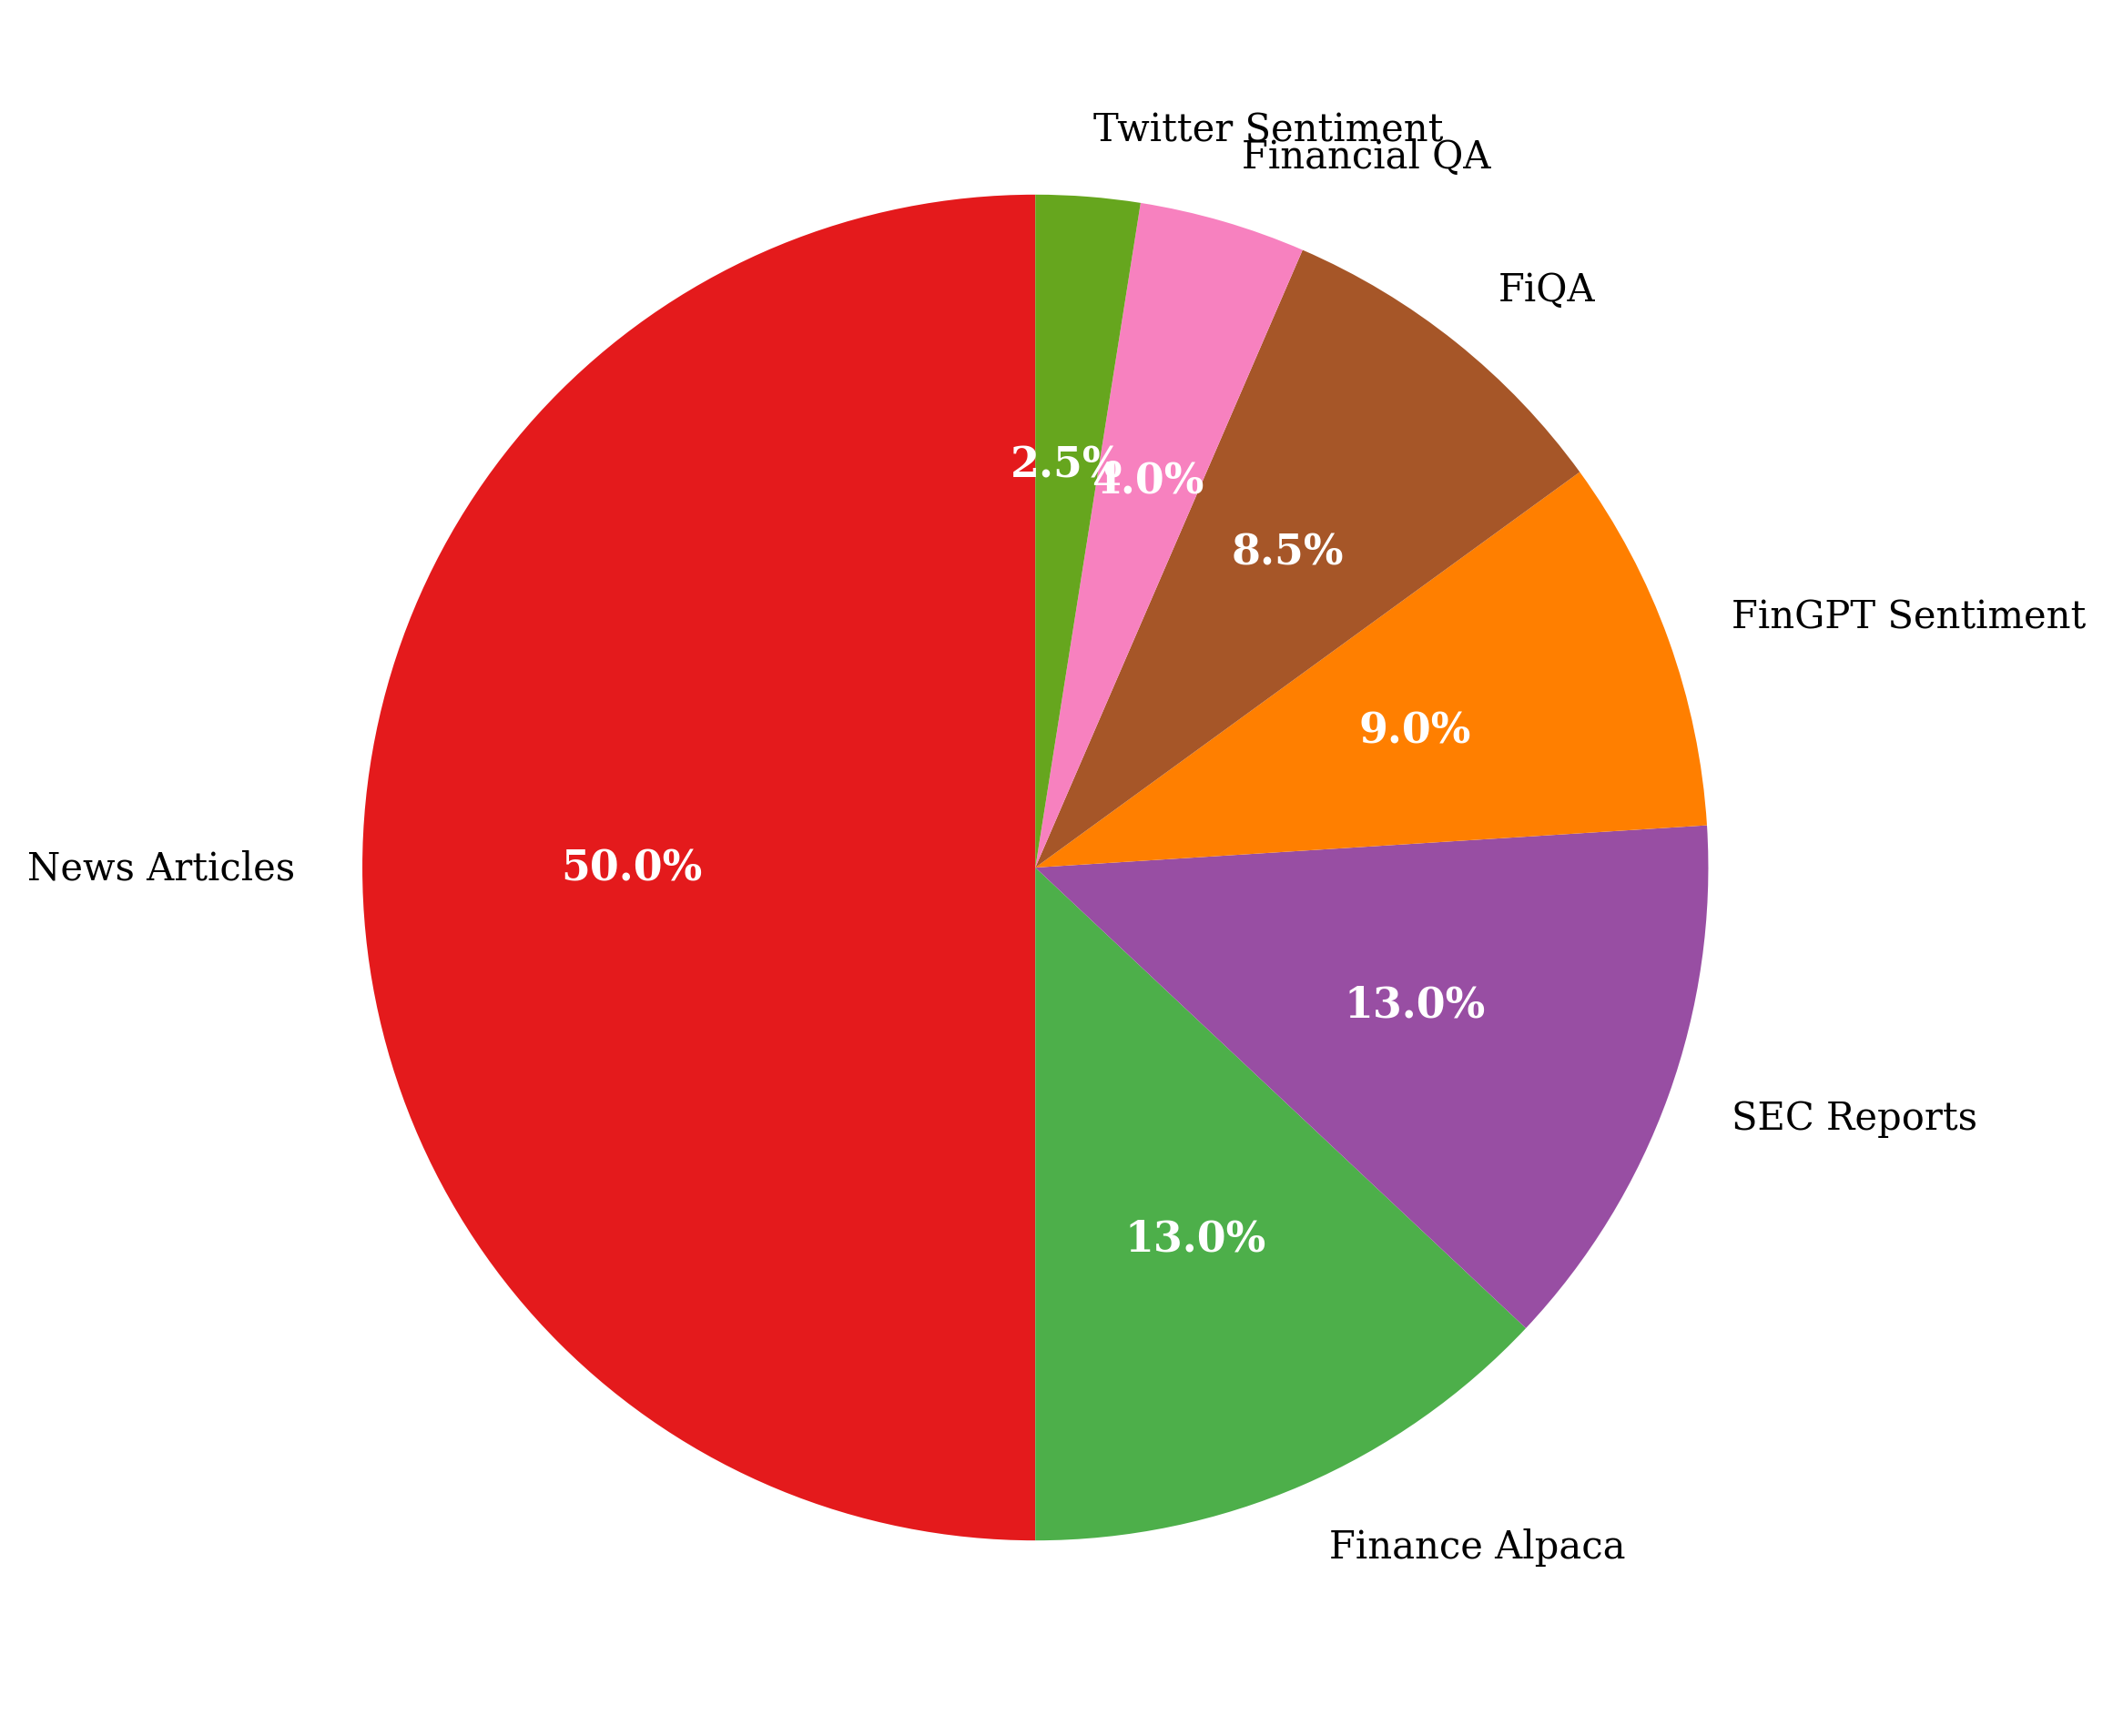
\includegraphics[width=0.95\textwidth]{figures/diagram_50cap.png}
\caption[Mixed Financial Token Budget]{100M token budget for Mixed Financial (7 datasets). Raw corpus: 219.77M tokens. After 50cap sampling: News 50.0M (50.0\%), Alpaca 13.0M (13.0\%), SEC 13.0M (13.0\%), FinGPT 9.0M (9.0\%), FiQA 8.5M (8.5\%), Financial QA 4.0M (4.0\%), Twitter 2.5M (2.5\%).}
\label{fig:diagram_50cap}
\end{figure}

\begin{figure}[htbp]
\centering
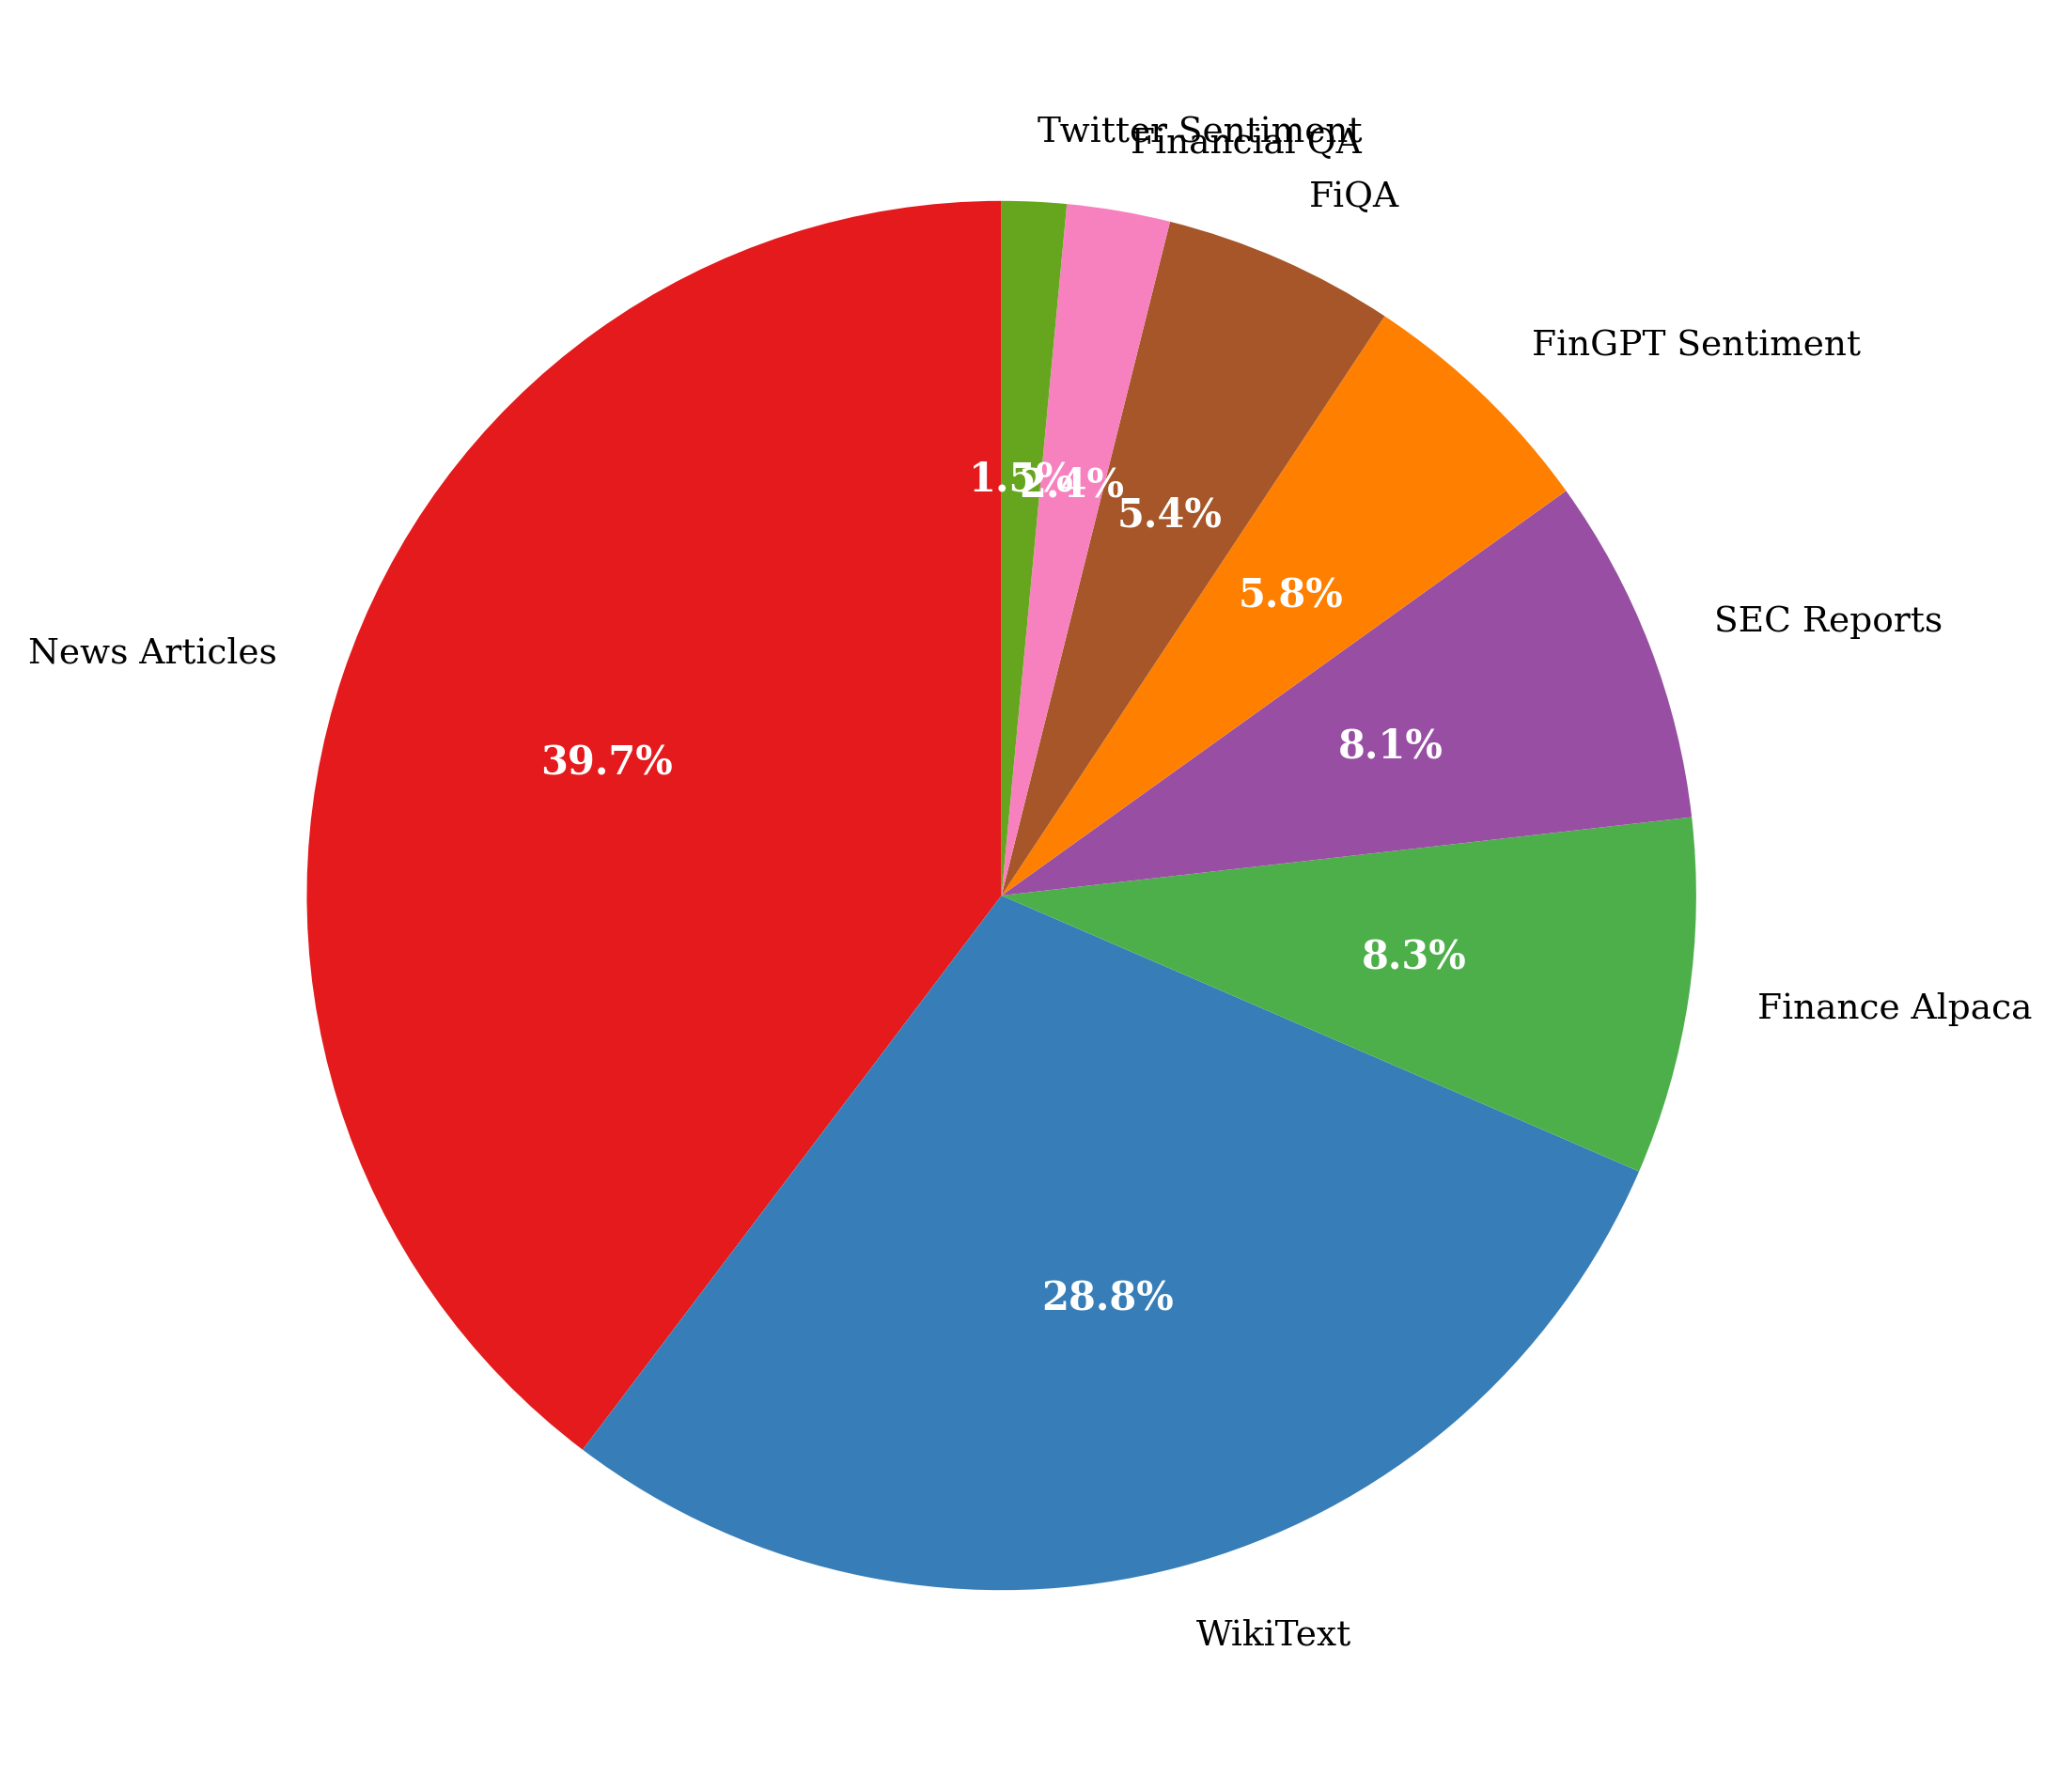
\includegraphics[width=0.95\textwidth]{figures/diagram_mixed_wiki.png}
\caption[Mixed Wiki+Financial Token Budget]{100M token budget for Mixed Wiki+Financial (8 datasets). Raw corpus: 343.35M tokens. After 50cap sampling: News 39.7M (39.7\%), WikiText 28.8M (28.8\%), Alpaca 8.3M (8.3\%), SEC 8.1M (8.1\%), FinGPT 5.8M (5.8\%), FiQA 5.4M (5.4\%), Financial QA 2.4M (2.4\%), Twitter 1.5M (1.5\%).}
\label{fig:diagram_mixed_wiki}
\end{figure}

\section{Training Setup and Hyperparameter Tuning}

\subsection{Initial Configuration}

We trained all models with a single hyperparameter template to set a baseline. 

We used AdamW ($\beta_1=0.9$, $\beta_2=0.999$, $\epsilon=10^{-8}$, weight decay $0.01$) with an initial learning rate of $2\times10^{-5}$, cosine decay, 1{,}000 warmup steps, and minimum LR $10^{-6}$. The effective batch size was 8 across all runs; when memory was tight, we used gradient accumulation to maintain that size. Sequences were 1{,}024 tokens with bfloat16 mixed precision. Training duration was dataset‑dependent: large datasets ($>$100M tokens) trained for $<$1 epoch (News: 0.5 epochs, WikiText: 0.8 epochs), medium datasets (3.6–8.5M) for 12–28 epochs, and small datasets ($<$1M) for 143–352 epochs to reach the fixed 100M token budget.

When we observed abnormalities in a few experiments, we reran those specific cases with smaller LRs as a simple heuristic to stabilize training.

\subsection{Pragmatic Learning Rate Adjustments}

In three configurations we observed abnormal behavior (e.g., larger models underperforming smaller ones). For these few cases, we retried with smaller learning rates (e.g., $1\times 10^{-5}$ or $5\times 10^{-6}$) purely as a practical heuristic to stabilize training. We do not propose or rely on a learning-rate scaling theory in this work. LR-comparison tables for the affected settings are reported in Chapter~4.

\subsection{Other Hyperparameters}

Beyond learning rate, we kept other hyperparameters consistent: effective batch size 8 (using gradient accumulation as needed), warmup of 1{,}000 steps (8\% of 12K total steps), and dropout 0.0. Training epochs varied by dataset size to normalize token exposure: small datasets (Twitter, Financial QA) needed 143–352 epochs to reach 100M tokens; medium ones (SEC, FiQA, FinGPT, Alpaca) 12–28 epochs; large ones (News, WikiText) 0.5–0.8 epochs. We fixed maximum sequence length at 1{,}024 tokens; although financial documents often exceed this, longer sequences increase memory quadratically, so we accepted truncation as a practical trade‑off.

\subsection{Computational Budget}

To ensure fair comparison across experiments, we normalized the token budget to 100M tokens per training run, regardless of dataset size or model scale. In total we ran 36 trainings: two mixture settings (Mixed Financial; Mixed Wiki+Financial), eight single‑dataset baselines (WikiText, Financial News, SEC, FinGPT, Finance Alpaca, FiQA, Financial QA 10K, Twitter), each at three sizes (0.6B/1.7B/4B) for 30 baselines, plus six follow‑ups with reduced learning rates on the three problematic datasets (WikiText, Financial QA, Twitter) to probe sensitivity at larger scales. The total computational cost was $36\times100\text{M}=3.6\text{B}$ tokens.

This token controlled design helps ensure that performance differences reflect model data interactions rather than unequal training compute. Variable epoch counts (2 to 249 across experiments) follow from dataset size while keeping token exposure constant. But it also means small datasets see many passes. We accept this trade-off for fair comparisons across different settings.

\section{Evaluation Protocol}

\subsection{Multi-Dataset Evaluation}

Each trained model is evaluated on eight held‑out test sets to measure both in‑domain and out‑of‑domain generalization: seven financial test splits (News, SEC, FinGPT, Alpaca, FiQA, Financial QA, Twitter) plus WikiText test split to evaluate general language capabilities and cross‑domain transfer.

For models trained on dataset $D$, evaluation on $D$'s test set measures in-domain generalization; evaluation on other datasets measures cross-dataset transfer. For mixed models, all 8 test sets measure generalization across the mixture distribution.

\subsection{Metrics}

We report three complementary metrics. We first use Cross‑entropy loss, which is the average negative log‑likelihood per token,
\begin{equation*}
    \mathcal{L} = -\frac{1}{N}\sum_{i=1}^{N} \log P\bigl(w_i \,\mid\, w_{<i}\bigr)
\end{equation*}
with lower being better. 

We then use \textbf{Perplexity} as a interpretable transformation, where $\text{PPL}=\exp(\mathcal{L})$. Lower PPL indicates better performance.

We also use \textbf{Relative Spread} to measure cross‑dataset variability:
\begin{equation*}
    \text{Relative Spread}\% = 100\,\frac{\max(\text{PPL}) - \min(\text{PPL})}{\text{mean PPL}}\, ,
\end{equation*}
computed over evaluation perplexities (one per dataset); lower values indicate more consistent generalization.

All metrics are computed on full test sets (no subsampling) with the same sequence length (1,024 tokens) and batch size used during training. Evaluation uses the final checkpoint from training (no checkpoint selection based on validation performance).
